\documentclass[12pt]{article}

\usepackage[margin=1in]{geometry}
\usepackage{amsmath,amsthm,amssymb}
\usepackage{nccmath}
\usepackage{mathtools}
\usepackage{mathrsfs}
\usepackage{enumitem}
\usepackage{physics}
\usepackage{slashed}
\usepackage{pdfpages}
\usepackage{float}

\usepackage{tikz}
\usepackage{tikz-feynman}

\graphicspath{ {./images/} }
\newcommand{\magsq}[1]{\big|#1\big|^2}

\begin{document}

\title{Homework 4}
\author{Sean Ericson \\ Phys 663}
\maketitle

\section*{Problem 1}
\begin{figure}[H]
    \centering
    \resizebox{0.65\textwidth}{!}{
        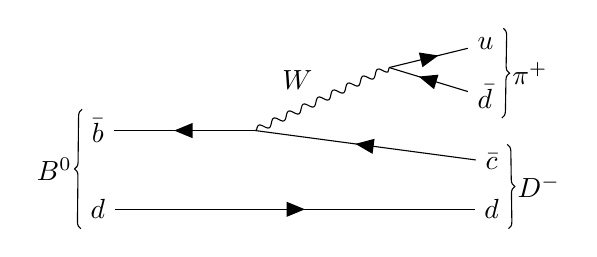
\begin{tikzpicture}
            \begin{feynman}
            \vertex (i2) {$d$}; 
            \vertex[above=1 of i2] (i1) {$\bar{b}$}; 
            \vertex[right=5 of i2] (f4) {$d$};
            \vertex[below right=.4 and 5 of i1] (f3) {$\bar{c}$};
            \vertex[right=2 of i1] (v1);
            \vertex[above right=.8 and 1.7 of v1] (v2);
            \vertex[above right=0.1 and 1 of v2] (f1) {$u$};
            \vertex[below right=0.1 and 1 of v2] (f2) {$\bar{d}$};
            \diagram* { {[edges=fermion]
            (i2) -- (f4),
            (f3) -- (v1) -- (i1), 
            (f2) -- (v2) -- (f1)},
            (v1) -- [boson, edge label=$W$] (v2)
            };
            \draw [decoration={brace}, decorate] (i2.south west) -- (i1.north west) node [pos=0.5, left] {$B^0$};
            \draw [decoration={brace}, decorate] (f1.north east) --  (f2.south east) node [pos=0.5, right] {$\pi^+$};
            \draw [decoration={brace}, decorate] (f3.north east) --  (f4.south east) node [pos=0.5, right] {$D^-$};
            \end{feynman} 
        \end{tikzpicture}
    }
    \caption{The decay $B^0 \to \pi^+ + D^-$.}
    \label{fig1}
\end{figure}
    \begin{figure}[H]
        \centering
        \resizebox{0.65\textwidth}{!}{
        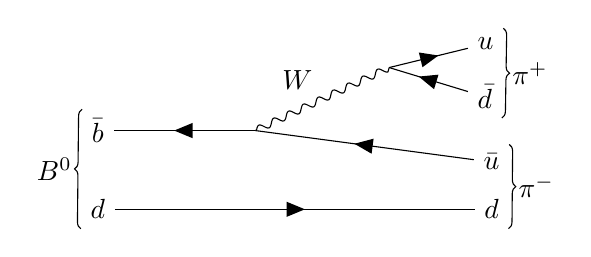
\begin{tikzpicture}
            \begin{feynman}
            \vertex (i2) {$d$}; 
            \vertex[above=1 of i2] (i1) {$\bar{b}$}; 
            \vertex[right=5 of i2] (f4) {$d$};
            \vertex[below right=.4 and 5 of i1] (f3) {$\bar{u}$};
            \vertex[right=2 of i1] (v1);
            \vertex[above right=.8 and 1.7 of v1] (v2);
            \vertex[above right=0.1 and 1 of v2] (f1) {$u$};
            \vertex[below right=0.1 and 1 of v2] (f2) {$\bar{d}$};
            \diagram* { {[edges=fermion]
            (i2) -- (f4),
            (f3) -- (v1) -- (i1), 
            (f2) -- (v2) -- (f1)},
            (v1) -- [boson, edge label=$W$] (v2)
            };
            \draw [decoration={brace}, decorate] (i2.south west) -- (i1.north west) node [pos=0.5, left] {$B^0$};
            \draw [decoration={brace}, decorate] (f1.north east) --  (f2.south east) node [pos=0.5, right] {$\pi^+$};
            \draw [decoration={brace}, decorate] (f3.north east) --  (f4.south east) node [pos=0.5, right] {$\pi^-$};
            \end{feynman} 
        \end{tikzpicture}
        }
        \caption{The decay $B^0 \to \pi^+ + \pi^-$.}
        \label{fig2}
    \end{figure}
    \begin{figure}[H]
    \centering
    \resizebox{0.65\textwidth}{!}{
        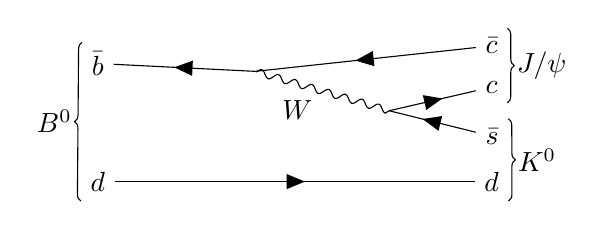
\begin{tikzpicture}
            \begin{feynman}
            \vertex (i2) {$d$}; 
            \vertex[above=1.5 of i2] (i1) {$\bar{b}$}; 
            \vertex[right=5 of i2] (f4) {$d$};
            \vertex[below right=0.1 and 2 of i1] (v1);
            \vertex[above right=.1 and 2.8 of v1] (f1) {$\bar{c}$};
            \vertex[below right=.5 and 1.7 of v1] (v2);
            \vertex[above right=0.1 and 1.1 of v2] (f2) {$c$};
            \vertex[below right=0.1 and 1.1 of v2] (f3) {$\bar{s}$};
            \diagram* { {[edges=fermion]
            (i2) -- (f4), (f1) -- (v1) -- (i1), (f3) -- (v2) -- (f2)},
            (v1) -- [boson, edge label'=$W$] (v2)
            };
            \draw [decoration={brace}, decorate] (i2.south west) -- (i1.north west) node [pos=0.5, left] {$B^0$};
            \draw [decoration={brace}, decorate] (f1.north east) --  (f2.south east) node [pos=0.5, right] {$J/\psi$};
            \draw [decoration={brace}, decorate] (f3.north east) --  (f4.south east) node [pos=0.5, right] {$K^0$};
            \end{feynman} 
        \end{tikzpicture}
    }
    \caption{The decay $B^0 \to J/\psi + K^0$.}
    \label{fig3}
\end{figure}
The decays contain factors of $V_{ud}V_{cb}^*$, $V_{ud}V_{ub}^*$, and $V_{cs}V_{cb}^*$, respectively. Using from Wikipedia the values
\[ \mqty(\abs{V_{ud}}&\abs{V_{us}}&\abs{V_{ub}}\\\abs{V_{cd}}&\abs{V_{cs}}&\abs{V_{cb}}\\\abs{V_{td}}&\abs{V_{ts}}&\abs{V_{tb}}) = \mqty(0.97373\pm0.00031&0.2243\pm0.0008&0.00382\pm0.00020\\0.221\pm0.004&0.975\pm0.006&0.0408\pm0.0014\\0.0086\pm0.0002&0.0415\pm0.0009&1.014\pm0.029), \]
the magnitudes of the factors above are given by $0.0397 \pm0.0014$, $0.00372\pm0.00019$, and $0.0398\pm0.0014$, respectively. The CKM factors for the first and third decays are similar in magnitude, but the additional charm quark in the final state should produce a phase space suppression. So, the first decay should be the most likely, followed by the third then the second.
The PDG gives branching ratios of $(2.51\pm0.08)\times10^{-3}$, $(5.12\pm0.19)\times10^{-6}$, and $(8.91\pm0.21)\times10^{-4}$, respectively. So, indeed, the first and last BR are of similar magnitudes, but the middle is down by a factor of 100ish.

\section{Problem 2}
\begin{enumerate}[label=(\alph*)]
    \item The integrated neutrino flux at the distance given is
    \[ \Phi_\nu = \frac{N_0}{4\pi R^2} = \frac{10^{58}}{4\pi(170,000\;\text{ly})^2} \approx 3\times10^{14}\;\text{m}^{-2}. \]
    Then, with a rough area of $A = (16 \text{m})^2$, the total number of neutrinos should be
    \[ N = A\Phi_\nu \approx 8\times10^{16}. \]

    \item The cross section should be proportional to the number of interactions that occurred, inversely proportional to the number of water molecules there are to interact with, and also inversely proportional to the integrated neutrino flux, i.e.
    \[ \sigma \sim \frac{N_\text{int}}{N_\text{water}\Phi_\nu}. \]
    The number of water molecules is roughly
    \[ N_\text{water} \approx N_A (16 m)^3 \rho_\text{water} / MM_\text{water} \approx 10^{32}. \]
    That gives a cross section of about $3\times10^{-6}$ pb, which is smaller than it should be by a couple orders of magnitude =/.

    \item From $E = m\gamma$, we know that 
    \[ m = E\sqrt{1 - v^2}. \]
    So, if we can get an estimate of the neutrinos' velocity, we could estimate their mass (given that their energy is ~1 MeV). However, since we don't know how long the light spent escaping the supernova, I'm not really sure how to use the given information to estimate the neutrino's velocity. Therefore, I'm going to think about the problem as if the neutrinos and photons left the supernova simultaneously, and the neutrinos arrived two hours after the light. \\
    Now, the travel times are given by
    \[ t_\gamma = \frac{d}{c}; \quad t_\nu = \frac{d}{v}. \]
    Solving for the velocity in terms of the time difference, we have
    \[ \Delta t = t_\gamma - t_\nu \implies v = \left(c^{-1} + \Delta t / d\right)^{-1}. \]
    Plugging this into the mass equation above, we find
    \[ m = 1\;\text{MeV}\;\sqrt{1 - \frac{1}{c^2}\left(c^{-1} + \frac{2\;\text{hour}}{170,000\;\text{ly}}\right)^2} \approx 52\;\text{eV}. \]
    That a PHAT neutrino. Using the only other quantity with dimensions of time (the one minute window over which the neutrinos were observed) in the place of the 2 hours in the equation above reduces the predicted mass to about 4eV, but using that length of time makes even less sense.
\end{enumerate}

\section{Problem 3}
\begin{enumerate}[label=(\alph*)]
    \item The flavor eigenstates of the neutrinos can be written in the mass basis as
    \[ \ket{\nu_\alpha(x)} = \sum_i e^{i\phi_i x}V_{\alpha i}\ket{\nu_i}; \qquad \phi_i \coloneqq E - \frac{m_i^2}{2E}. \]
    The overlap between the flavor eigenstate $\beta$ at position $x$ with an initial flavor $\alpha$ is given by
    \begin{align*}
        \braket{\nu_\beta(x)}{\nu_\alpha(0)} &= \sum_{ij} e^{-i\phi_ix}V_{\beta i}^*V_{\alpha j}\braket{\nu_i}{\nu_j} \\
        &= \sum_i e^{-i\phi_i x}V_{\beta i}^* V_{\alpha i}.
    \end{align*}
    The desired probability is then
    \begin{align*}
        P(\nu_\alpha \to \nu_\beta) &= \magsq{\braket{\nu_\beta(x)}{\nu_\alpha(0)}} \\
        &= \magsq{\sum_i e^{-i\phi_i x}V_{\beta i}^* V_{\alpha i}} \\
        &= \sum_{ij}e^{-i\Delta m_{ij}^2/2E} z_{\alpha\beta;ij},
    \end{align*}
    where
    \[ z_{\alpha\beta;ij} \coloneqq V_{\alpha i}^*V_{\alpha j}V_{\beta i}V_{\beta j}^* \]
    Ahhhghghg sorry, this is driving me crazy! I've tried going at this in a few different ways and I can't seem to make it work out. I'm pretty sure I should separate out the $i=j$ terms, then pair up the $i\neq j$ terms, but I can't seem to get a $2\sin^2 - \sin$ out of that.

    \item 
    \begin{align*}
        \sum_\beta P(\nu_\alpha \to \nu_\beta) &= \sum_\beta\left(\delta_{\alpha\beta} - 2\sum_{i>j}\left(2\sin^2\frac{\Delta m_{ij}^2}{4E}\Re[z_{\alpha\beta;ij}] - \sin\frac{\Delta m_{ij}^2}{2E}\Im[z_{\alpha\beta;ij}]\right)\right) \\
        &= 1 - 2\sum_{i>j}\left(2\sin^2\frac{\Delta m_{ij}^2}{4E}\Re[\sum_\beta z_{\alpha\beta;ij}] - \sin\frac{\Delta m_{ij}^2}{2E}\Im[\sum_\beta z_{\alpha\beta;ij}]\right) \\
        &= 1 - 2\sum_{i>j}\left(2\sin^2\frac{\Delta m_{ij}^2}{4E}V_{\alpha i}^*V_{\alpha j}\delta_{ij} - \sin\frac{\Delta m_{ij}^2}{2E}V_{\alpha i}^*V_{\alpha j}\delta_{ij}\right) \\
        &= 1
    \end{align*}
    The second line follows from linearity of the sum, the third equality follows from the unitarity of the PMNS matrix, and the last equality follow from the sum having no terms with $i=j$.

    \item For $\alpha = \beta$, we have that
    \[ z_{\alpha\alpha;ij} = V_{\alpha i}^*V_{\alpha j}V_{\alpha i}V_{\alpha j}^* = \magsq{V_{\alpha i}}\magsq{V_{\alpha j}} \in \mathbb{R}, \]
    so clearly the $\Im[z_{\alpha\alpha;ij}]$ term vanishes. In the case that $m_3^2 \gg m_1^2,\;m_2^2$, we have that 
    \[ \Delta m_{13}^2 \approx \Delta m_{23}^2 \gg \Delta m_{12}^2 \]
    Approximating
    \[ \Delta m_{13}^2 = \Delta m_{23}^2 \eqqcolon \Delta m^2 \]
    \[ \Delta m_{12}^2 = 0, \]
    we have that
    \[ P(\nu_\mu \to \nu_\mu) \approx 1 - 4\sin^2\frac{\Delta m^2}{4E}\left(\magsq{V_{\mu 1}V_{\mu 3}} + \magsq{V_{\mu 2}V_{\mu 3}}\right). \]
    Comparing this to the probability given in Peskin for the two neutrino model,
    \[ P(\nu_\mu \to \nu_\mu) = 1 - \sin^22\theta\sin^2\frac{\delta m^2}{4E}, \]
    we se that they agree given
    \begin{align*}
        \delta m^2 &= \Delta m^2 \\
        \sin^22\theta &= 4\left(\magsq{V_{\mu 1}V_{\mu 3}} + \magsq{V_{\mu 2}V_{\mu 3}}\right)
    \end{align*}
\end{enumerate}

\end{document}